\chapter{Einführung}

Unter den 25 häufigsten Todesursachen weltweit sind drei Krebsarten vertreten, eine davon ist Darmkrebs~\cite{Lozano.2012}.
Sie hat die vierthöchste Sterblichkeitsrate von allen Krebsarten~\cite{Ferlay.2012} und liegt etwa 10~\% aller Krebstode zugrunde~\cite{Kumar.2005}.
Polypen in der Darmschleimhaut bilden dessen Vorstufe~\cite{Kumar.2005}.
Eine frühzeitige Entfernung bösartiger Kolorektalpolypen kann das Sterblichkeitsrisiko bis zur Hälfte reduzieren~\cite{Zauber.2012}, während die vollständige Resektion sämtlicher sowohl benigner als auch maligner Polypen unnötige Risiken wie Blutungen und Perforation aufweisen~\cite{Rex.2009}.

Regelmäßige Vorsorgeuntersuchungen ermöglichen es, das Wachstum von Kolorektalpolypen zu überwachen.
Hierbei wird in der Regel der Dickdarm im Rahmen einer Koloskopie endoskopisch untersucht~\cite{Kumar.2005} und von verdächtigen Polypen wird eine Gewebeprobe genommen, um diese anschließend histologisch auf ihre Gut- oder Bösartigkeit zu untersuchen.

Bei solchen Darmspiegelungen werden oftmals bis zu 28~\% aller Polypen übersehen~\cite{Leufkens.2012}.
Mit einer Markierung im endoskopischen Bild wie in \autoref{fig:highlight} könnte man Ärzten das Auffinden von Polypen erleichtern und die Fehlerrate verringern.
Grundlage dafür wäre eine automatische Lokalisierung von Polypen im koloskopischen Bild (s. \autoref{fig:segm}).

\begin{figure}
	\centering
	\begin{subfigure}{.3\textwidth}
		\centering
		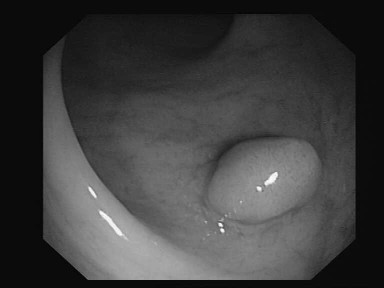
\includegraphics[width=.8\linewidth]{polyp129}
		\caption{}
		\label{fig:polyp}
	\end{subfigure}
	\begin{subfigure}{.3\textwidth}
		\centering
		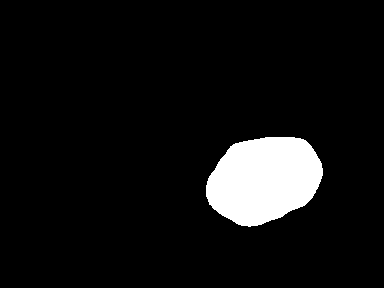
\includegraphics[width=.8\linewidth]{segm129}
		\caption{}
		\label{fig:segm}
	\end{subfigure}
	\begin{subfigure}{.3\textwidth}
		\centering
		% TODO Create graphic
		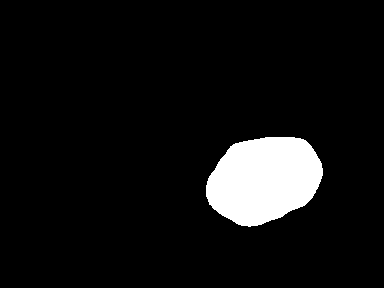
\includegraphics[width=.8\linewidth]{segm129}
		\caption{}
		\label{fig:highlight}
	\end{subfigure}
	\caption{Kolorektalpolyp, dessen Segmentierung und Hervorhebung im Bild~\cite{Vazquez.2017}}
	\label{fig:polypseg}
\end{figure}

In der vorliegenden Masterarbeit wird zur Lösung dieses Lokalisierungsproblems ein Deep-Learning-Ansatz verwendet, der bisher noch nicht bei der Lokalisierung von Polypen eingesetzt wurde.
Dieser Ansatz, die \glspl{can} \cite{Isola.2017}, basiert auf den \glspl{gan} \cite{Goodfellow.2014}.

Dieses Kapitel erläutert die Problemstellung und stellt den Stand der Technik vor.
In den anschließenden Kapiteln erfolgt eine methodische Aufschlüsselung des Vorgehens in dieser Arbeit, die Umsetzung dieser Methodik, deren Ergebnisse und eine Analyse dieser Ergebnisse.



\section{Medizinischer Hintergrund}

\emph{Polypen} beginnen generell als leichte Erhebungen in der Schleimhaut, die in das Lumen des umgebenden Organs hineinragen~\cite{Kumar.2005}.
Anfangs wachsen sie \emph{sessil} ("stiellos") und sind nur als breite Kuppeln sichtbar, können aber im Lauf der Zeit einen Stiel entwickeln, sodass \emph{gestielte} Polypen in etwa pilzförmig aussehen.

Polypen lassen sich einteilen in \emph{neoplastisch} und \emph{nicht-neoplastisch}~\cite{Kumar.2005}.
Die häufigste neoplastische Polypenform ist das \emph{Adenom}, das sich im Laufe der Zeit zu Krebs entwickeln kann.
Alle anderen Polypenarten hingegen entwickeln sich fast ausschließlich gutartig.
Das Aussehen eines Polyps reicht in der Regel nicht aus zur Beurteilung der Malignität; dies ist bisher fast ausschließlich durch eine histologische Untersuchung des Polypengewebes möglich.
Allerdings steigt mit zunehmender Größe eines Polypen die Wahrscheinlichkeit, dass es sich um ein Karzinom handelt.

Karzinome, die sich aus Adenomen entwickeln, sogenannte \emph{Adenokarzinome}, sind die häufigste Form von bösartigen Tumoren im \gls{gi}~\cite{Kumar.2005}.
Im Kolorektalbereich, der vom allerletzten Abschnitt des Dünndarms bis zum Rektum reicht, tritt die stark überwiegende Mehrheit aller malignen Polypen im \gls{gi} auf.
Im Dünndarm hingegen treten sowohl benigne als auch maligne Polypen sehr selten auf; die Auftrittswahrscheinlichkeit sinkt weiter, je höher man im \gls{gi} aufsteigt.
In dieser Arbeit wird deshalb ausschließlich die Segmentierung von \emph{Kolorektalpolypen} betrachtet.

Zur Untersuchung des Kolorektalbereichs wird üblicherweise eine Koloskopie durchgeführt, bei der mittels eines rektal eingeführten Endoskops die gesamte Region inspiziert werden kann.
Analog dazu werden bei einer Spiegelung des Dünndarms meist oral eingeführte Endoskopkapseln eingesetzt, was als \gls{wce} bezeichnet wird.
Im Kontext dieser Arbeit wird nur auf Bildmaterial eingegangen, das durch Endoskopie im Bereich des sichtbaren Lichts produziert wurde.
Andere Modalitäten wie bspw. Narrow Band Imaging, bei dem zur besseren Hervorhebung bestimmter Gewebsarten nur bestimmte schmale Frequenzbänder des sichtbaren Lichts zum Einsatz kommen, werden hier nicht betrachtet.



\section{Problemstellung}

Um eine Hervorhebung von Polypen im koloskopischen Bild während einer Darmspiegelung zu ermöglichen, ist ein automatisiertes Auffinden von Polypen notwendig.
Diese Lokalisierung kann unterschiedlich genau sein, vom einzelnen Bildpunkt über Bounding Boxes bis hin zu ellipsenförmigen Bereichen.
Wenn ein Algorithmus in der Lage ist, die Fläche des Polypen \emph{pixelgenau} im Bild zu finden, wird in dieser Arbeit von einer \emph{Segmentierung} gesprochen als der genauesten Form der Lokalisierung.
In allen anderen Fällen wird nur von einer \emph{Lokalisierung} gesprochen.

Diese Arbeit befasst sich mit dem Einsatz einer bestimmten Deep-Learning-Architektur, um Polypen in koloskopischen Bildern zu segmentieren.
Dabei soll sowohl die Qualität der Segmentierung als auch Verbesserungen zur Stabilisierung des Trainings evaluiert werden.
In den folgenden Abschnitten werden alternative, bereits bestehende Ansätze zur Polypen-Lokalisierung und -Segmentierung vorgestellt und erläutert.
Diese werden hier aufgeteilt in solche Ansätze, bei denen die relevanten Bildmerkmale vom menschlichen Experten festgelegt werden, und solche, bei denen Features vollständig gelernt werden.

In Echtzeitszenarien kann es durchaus sinnvoll sein, zuerst einen leichtgewichtigeren Algorithmus binär detektieren zu lassen, ob ein Polyp im Bild vorhanden ist, und anschließend diese \emph{Präsenz-Detektion} durch eine Lokalisierung zu erweitern.
Im Rahmen dieser Arbeit werden Methoden zur reinen Detektion der Präsenz von Polypen allerdings nicht genauer betrachtet.

Ebenso ist die Beurteilung der Bösartigkeit des Gewebes anhand der Bildinformation, eine sogenannte "optische Biopsie", zwar ein interessantes Forschungsproblem~\cite{Roy.2011}, aber diese Arbeit hat keine derartige Klassifikation zum Ziel.
%TODO optical biopsy als Ausblick am Schluss



\section{Feature Selection}

Algorithmen, die Bilder verarbeiten, haben es in aller Regel mit sehr hochdimensionalen Daten zu tun.
Aus diesen Eingabedaten wird versucht, gehaltvolle Ausgaben zu erzeugen wie bspw. Aussagen über die Präsenz gewisser Objekte, menschliche Emotionen oder die Position bestimmter Objekte.
Um aus diesen hochdimensionalen Inputs Ausgaben mit deutlich geringerer Dimensionalität zu erzeugen, ist es notwendig, die Dimensionalität des Inputs zu reduzieren, indem man Merkmale verwirft, die für die Ausgabe nicht relevant sind.

Woher weiß der Algorithmus, welche Merkmale relevant sind?
Entweder man instruiert ihn explizit, indem man Expertenwissen fest in den Algorithmus einkodiert, oder man lässt es ihn selbstständig herausfinden.
Die erste Variante produziert zumeist Algorithmen, die sehr auf Problem und Domäne zugeschnitten und nur schwer übertragbar sind; allerdings kann man die Kriterien, anhand derer sie eine Ausgabe erzeugen, von außen nachvollziehen.
Die zweite Variante hingegen erzeugt Algorithmen, die große Mengen an Trainingsdaten benötigen, dafür aber tendentiell viel flexibler und einfacher auf andere Domänen übertragbar sind.

In diesem Abschnitt werden Ansätze zur Lokalisierung und Segmentierung von Polypen vorgestellt, die zur ersten Kategorie gehören; im darauffolgenden Abschnitt folgen Ansätze der zweiten Kategorie.



\subsection{Lokalisierung}

In \cite{Prasath.2016} reviewt \citeauthor{Prasath.2016} verschiedene Ansätze zur Detektion, Lokalisierung und Segmentierung von Polypen in \gls{wce}-Videos.
Auch wenn die Gegebenheiten der Bildgebung bei der Kapselendoskopie sich von denen der Koloskopie unterscheiden, arbeiten doch beide im Spektrum des sichtbaren Lichts, weshalb ein Vergleich von Algorithmen beider Modalitäten möglich sein sollte.

Auch wenn Ansätze zur reinen Detektion von Polypen hier nicht genauer betrachtet werden, bauen doch die Mehrheit solcher Ansätze einen Lokalisierungsschritt ein, um dann zu entscheiden, ob ein Polyp im Bild vorhanden ist~\cite{Prasath.2016}.
Bei solchen Lokalisierungen kommen meist elliptische Features, Textur, Farbe und Positionseigenschaften als Merkmale zum Einsatz.

Von den bei \cite{Prasath.2016} vorgestellten Ansätzen verlassen sich die meisten Lokalisierungen auf die Filterung von Kanten und eigens gefertige Maße für Krümmungen und Vorwölbungen im Bild.
Mithilfe dieser Features werden Lokalisierungen erzielt, die als Ausgabe einen Bildpunkt, eine Bounding Box, eine Ellipse oder eine grobe Segmentierung erzielen.
Oftmals kommen im Ablauf einzelner Algorithmen gelernte Elemente hinzu wie bspw. ein Clustering-Algorithmus zur Filterung von Lokalisierungskandidaten, aber dennoch werden die Merkmale, auf denen gelernt wird, vom Menschen ausgewählt.

Abgesehen von den in \cite{Prasath.2016} verglichenen Ansätzen geht folgende Arbeit ebenfalls dem Lokalisierungsbroblem nach:
In \cite{Li.2004} ist das Ziel eine Lokalisierung von abnormalen Regionen im koloskopischen Bild, wozu auch Regionen mit Polypen zählen.
Ausgabe ist eine binäre Segmentierung mit rechtwinkligen Grenzen, da mit Patches des Bildes gearbeitet wird, von denen jeder einzeln mittels eines Ensemble-Lerners klassifiziert wird.
Diese Patches werden auf mehreren Skalierungen erstellt, um verschiedene Abnormalitätengrößen erfassen zu können.
Features in den einzelnen Patches werden generiert durch eine Diskretisierung der Farbwerte im CIELab-Farbraum und anschließende Berechnung von Farb-Features und -Statistiken, die u.~a. von einer diskreten Wavelet-Transformation stammen.



\subsection{Segmentierung}

Bei \cite{Prasath.2016} werden auch verschiedene Segmentierungsalgorithmen für Kolorektalpolypen verglichen.
Diese basieren alle auf Varianten von \emph{Active Contours}~\cite{Kass.1988}, bei denen ein verformbares, a priori festgelegtes Linienmodell durch Energieminimierung auf ein Bild eingepasst wird.
\citeauthor{Sasmal.2018} nutzen ebenfalls Active Contours und initialisieren die Segmentierung mit kreisförmigen Löchern auf die gesamte Bildfläche~\cite{Sasmal.2018}.

\citeauthor{Ionescu.2013} halten die gekrümmte Form der Polypen für am meisten aussagekräftig und entwickeln eine eigene Methode zur Verstärkung der Polypenkanten im Bild~\cite{Ionescu.2013}.
\citeauthor{Vieira.2012} segmentieren abnormales Gewebe von normalem und nutzen dafür ein Gaussian Mixture Model basierend auf den Vektoren im HSV- und RGB-Farbraum~\cite{Vieira.2012}.




\section{Feature Learning}

Kolorektalpolypen zu lokalisieren ist komplex, denn Form, Textur und Farbe unterscheiden sich teilweise drastisch zwischen Polypen, oftmals sogar beim selben Patienten~\cite{Prasath.2016}.
Viele der vorgestellten Lokalisierungsverfahren nutzen Kombinationen dieser Features, aber die Segmentierungsverfahren verlassen sich alle ausschließlich auf die Form als entscheidendes Merkmal (bis auf einen rein farbbasierten Ansatz).
Aufgrund der hohen Varianz an Polypenaussehen kann es nicht ausreichen, sich nur auf eines dieser Merkmale zu verlassen~\cite{Prasath.2016}.

Algorithmen, die selbst explorativ herausfinden, welche Features relevant sind, lernen auf den originalen Rohdaten und können somit jegliche Kombination aus Merkmalen zur Lösung des Problems nutzen.
Die Ansätze in diesem Abschnitt basieren alle auf Feature Learning.
\emph{Deep Learning} ist hierbei das Konzept, das Feature Learning bisher am erfolgreichsten ganzheitlich inkorporiert.
Anders als bestimmte Clusteringverfahren oder die \gls{pca}~\cite{Hotelling.1933}, die sich darauf beschränken aussagekräftige Merkmale zu finden, ermöglicht Deep Learning nicht nur das Erlernen von Features, sondern auch das Lernen von Mappings von Merkmalswerten zu gewünschten Ausgaben.

Deep Learning bezeichnet eine Klasse von Algorithmen, bei denen künstliche \glspl{nn} zum Einsatz kommen, die mehr als eine verborgene Schicht besitzen~\cite{Goodfellow.2016}.
Viele lernende Algorithmen kommen nur mit Problemen in niedrigdimensionalen Räumen zurecht, weil sie theoretisch für jeden möglichen Punkt im Merkmalsraum Trainingsbeispiele benötigen.
Abgesehen von diesem "Fluch der Dimensionalität"~\cite{Bellman.2010} stützen sich viele Lernalgorithmen auf die Annahme, dass die zu lernende Funktion in kleinen, lokalen Bereichen ungefähr konstant verläuft, was aber nicht immer der Fall sein muss.
Beiden Problemen kann Deep Learning entgegentreten durch das Lernen von niedrigdimensionalen, nicht-lokalen Mannigfaltigkeiten im Merkmalsraum~\cite{Bengio.2005} und durch die Annahme, dass die Trainingsdaten durch mehrere zugrundeliegende Faktoren, möglicherweise auf mehreren Abstraktionsebenen, verursacht wurden~\cite{Goodfellow.2016}.
Gerade letztere Hypothese bietet sich sehr gut für das hier vorliegende Segmentierungsproblem an, da das Zusammenwirken verschiedener Faktoren eine Grundannahme ist.

Generell bieten Features lernende Algorithmen einen weiteren Vorteil gegenüber solchen mit selektierten Features:
Es ist kaum Vorverarbeitung notwendig, da der Algorithmus selbstständig lernt, welche Informationen des Originalinputs nicht relevant sind.
Aufwendiges Entfernen von Glanzlichtern oder das Limitieren des Gesamtbildes auf eine Interessenregion entfällt, was gerade bei den Ansätzen im vorherigen Abschnitt sehr häufig eingebaut wird.



\subsection{Convolutional Neural Networks}

Eine Deep-Learning-Architektur, die besonders im Bereich der Bildverarbeitung sehr verbreitet ist, ist das \gls{cnn}.
In dieser Variante von tiefen \glspl{nn} wird in mindestens einer Schicht die Faltungsoperation angewandt.
Die Werte einer Kernelmatrix, die für eine Neuronenschicht in jedem Bildfenster gleich bleibt, werden vom Netz gelernt.
Da die Neuronen in \glspl{cnn} mehr Parameter untereinander teilen als Netze mit vollständig verbundenen Schichten, die einer Matrixmultiplikation entspricht, ist ihre Speicherkomplexität geringer.

Durch den Einsatz von Pooling-Schichten oder Faltungsschichten mit größeren Strides sind \glspl{cnn} außerdem in der Lage, Repräsentationen zu lernen, die gegenüber kleinen Verschiebungen im Input invariant sind.
Dies wiederum drückt eine A-Priori-Annahme in \glspl{cnn} aus, die sich für Bilder sehr gut eignet:
Geringe Translationen sollten die Semantik eines Bildes nicht verändern.

Damit \glspl{cnn} gut generalisieren, benötigen sie in der Regel sehr viele Trainingsdaten.
In vielen Fällen lässt sich ein Netz, das schon für ein bestimmtes Problem trainiert wurde, als Ausgangspunkt für ein neues Netz nehmen, welches das bereits trainierte Netz nur noch leicht anpassend nachtrainiert auf das neue Zielproblem.
Dieses \emph{Transfer Learning} kann den Bedarf an Trainingsdaten deutlich verringern.
Gerade im Bereich der Objekterkennung haben sich viele Deep-Learning-Architekturen etabliert, die auf großen, gelabelten Bilddatenbanken wie ImageNet~\cite{Deng.2009} trainiert wurden und deren erste Schichten gerne als Startpunkt für neue Objekterkennungsnetze in speziellen Domänen genutzt werden (s. z.~B.~\cite{Simonyan.2014}).
Im Kontext der medizinischen Bildverarbeitung wurde gezeigt, dass der Transfer bereits gelernter Netzwerte mit anschließendem Fine-Tuning mindestens so gute Ergebnisse liefert wie ein Netz, das von Grund auf trainiert wird~\cite{Tajbakhsh.2016}.



\subsection{Lokalisierung}

\citeauthor{Billah.2017} setzen bei ihrer Polypenlokalisierung auf eine Hybridlösung aus selbst gewählten und gelernten Merkmalen:
Die Features werden sowohl aus Wavelet-Transformationen~\cite{Mallat.1989} als auch von einem \gls{cnn} generiert~\cite{Billah.2017}.
Hierbei wird ein Sliding Window mit fester Größe über ein zu untersuchendes Bild gefahren und in jedem Fenster werden Features extrahiert.
Diese gelernten Features werden mithilfe einer \gls{svm} beurteilt, um zu entscheiden, ob das aktuelle Bildfenster einen Polypen enthält oder nicht; im Grunde genommen betreibt dieser Ansatz also Polypendetektion mit einem Sliding Window.
Wird ein Fenster gefunden, das einen Polypen enthält, wird die Lokalisierung noch etwas verfeinert und danach wird kein weiteres Bildfenster verarbeitet; es kann also maximal ein Polyp im Bild gefunden werden.

Die Extrahierung der Features geschieht zum einen mithilfe einer Wavelet-Transformation, die eine Mischung aus Farb- und Texturinformationen über mehrere Skalen des Bildfensters generiert und von denen mehrere statistische Werte berechnet und als Features genutzt werden, zum anderen werden Features eines \gls{cnn} dazu genommen.
Das \gls{cnn} wird so trainiert, dass es in der Lage ist, zwischen Polypen- und Nicht-Polypen-Frames zu unterscheiden; anschließend wird das gesamte \gls{cnn} bis auf seine allerletzte Klassifikationsschicht als Feature-Extraktor mitverwendet.

Leider zeigen die Autoren nicht auf, welchen Vorteil die Kombination der beiden Feature-Extraktoren bietet.
\glspl{cnn} arbeiten auf mehreren Skalen, entweder durch Pooling oder Strides größer als 1, und sie arbeiten auf dem originalen Rohmaterial und können deshalb ebenfalls sehr viele Zusammenhänge lernen.
Die Faltungsoperation in \glspl{cnn} macht es natürlich schwierig, Beziehungen zwischen Bildpunkten zu modellieren, die sehr weit entfernt sind -- eventuell bieten hier die vorgeschlagenen Farb-Textur-Wavelets Vorteile, die aber nur im einzelnen Vergleich ersichtlich wären.

\citeauthor{Lequan.2017}~\cite{Lequan.2017} sind die ersten, die ein \gls{fcn}~\cite{Long.2015} einsetzen zur Lokalisierung von Kolorektalpolypen.
\glspl{fcn} sind eine Weiterentwicklung von \glspl{cnn}, in denen es nur noch Faltungsschichten gibt und keinerlei Pooling oder vollständig verbundene Schichten mehr.
Außerdem wird zusätzlich zum Downsampling ein Upsampling gelernt, bei dem Informationen aus den vorherigen Skalierungsstufen des Netzes den Entfaltungs-Schichten durch Skip Connections zur Verfügung gestellt werden.
Die FCN-Variante mit Skip Connections auf den meisten Skalierungen ist auch diejenige, die am weitesten verbreitet ist, und nennt sich \emph{FCN-8s}.

Diese Architektur wurde ursprünglich entwickelt, um Segmentierungen zu lernen; in diesem Szenario wird allerdings nur eine Karte mit Wahrscheinlichkeiten generiert, wo im Bild sich wohl Polypen befinden.
Die Maximalpunkte dieser Karte sind die Ausgabe.
Interessanterweise verwenden \citeauthor{Lequan.2017} ein 3D-FCN, um auf Videosequenzen zu lernen und zu prädizieren, indem sie eine Videosequenz als ein 3D-Volumen auffassen und dann darauf 3D- statt 2D-Faltung betreiben, um neben räumlichen auch zeitliche Zusammenhänge zu erfassen.



\subsection{Segmentierung}

\glspl{fcn} und Erweiterungen davon sind auch bereits für Polypensegmentierung ausgiebig eingesetzt worden.
\citeauthor{Brandao.2017}~\cite{Brandao.2017} funktionieren drei populäre CNN-Architekturen zu \glspl{fcn} um, darunter AlexNet~\cite{Krizhevsky.2012}, GoogLeNet~\cite{Szegedy.2015} und VGGNet~\cite{Simonyan.2014}.
Jede dieser Architekturen wird in ein \gls{fcn} konvertiert, indem vollständig verbundene Schichten durch Faltungsschichten mit einem 1$\times$1-Kernel ersetzt werden und eine Entfaltungsschicht am Schluss hinzugefügt wird, um die grobe Ausgabe der vorherigen Schichten zu verfeinern.
In jeder zum \gls{fcn} konvertierten Architektur werden die vortrainierten Werte der jeweiligen Ursprungsarchitekturen verwendet und im Training auf einen Datensatz zur Polypensegmentierung genauer gelernt.
Das \gls{fcn} auf Basis von VGGNet schneidet hierbei am besten ab.

\citeauthor{Vazquez.2017}~\cite{Vazquez.2017} legen einen Benchmark zur Polypensegmentierung vor, indem sie zwei öffentliche Datasets kombinieren, sie durch eigene Annotationen erweitern und das FCN-8s~\cite{Long.2015} auf diesen Daten trainieren.
Neben den schon gekennzeichneten Polypenregionen in den Bildern maskieren diese Annotationen explizit den Hintergrund, das Lumen des Darms und Glanzlichter.
Ausgiebige Dataset Augmentation kommt zum Einsatz, darunter Zoom, Rotation, Scherung und Warping; am besten schneidet die Kombination aller vier Augmentierungstechniken ab.
Als Vergleich ziehen die Autoren jeweils einen State-of-the-Art Algorithmus mit manuell gewählten Features heran, der in der Lage ist entweder Polypen, Lumen oder Glanzlichter zu segmentieren.
Abgesehen von dem Algorithmus, der Glanzlichter segmentiert, liefert ein FCN-8s, das mit allen vier Klassen trainiert wird, bessere Ergebnisse als jeder der Algorithmen mit Feature Selection.
Gleichzeitig ist das FCN-8s in der Lage alle Klassen gleichzeitig zu segmentieren und dies in 88 ms zu bewerkstelligen, was weniger als 2~\% der Zeit sind, die der schnellste der drei Algorithmen für seine einzelne Klasse alleine genommen benötigt.

\citeauthor{Wichakam.2018}~\cite{Wichakam.2018} verbessern diese Vorlage hinsichtlich der Geschwindigkeit, indem sie das \gls{fcn} komprimieren.
Dies geschieht durch Auslassen und Zusammenfassen einiger Schichten mit 1$\times$1-Faltung.
Zusätzlich transferieren sie vortrainierte Werte von VGGNet und passen außerdem die Verlustfunktion an:
Statt der verbreiteten Kreuzentropie nutzen sie eine differenzierbare Variante des Dice-Score~\cite{Srensen.1948}, der nur die Polypen-Klasse betrachtet und die Hintergrund-Klasse außer Acht lässt.
Mit diesen Maßnahmen erreichen die Autoren Ergebnisse, die in allen verwendeten Metriken weniger als einen Prozentpunkt schlechter sind als die des FCNs von \citeauthor{Vazquez.2017} und gleichzeitig nur 8 ms zur Inferenz benötigen.

\citeauthor{Wang.2018c} \cite{Wang.2018d,Wang.2018b,Wang.2018,Wang.2018c} setzen ebenfalls \glspl{fcn} und einige davon inspirierte Deep-Learning-Architekturen ein, darunter U-Net~\cite{Ronneberger.2015}, SegNet~\cite{Badrinarayanan.2017} und eine nicht näher erläuterte Variante von ResNet (Original s. \cite{He.2016}).
Eines ihrer U-Net-Experimente beinhaltet eine ausführliche Vorverarbeitung des Bildinputs und Nachverarbeitung des Netz-Outputs, ein anderes benötigt keinerlei Bereinigung.
Insgesamt schneidet das modifizierte ResNet am besten ab, aber die Ergebnisse sind schwer zu beurteilen, da bisher nur Abstracts veröffentlicht wurden.



\subsection{Generative Netze}

\glspl{cnn} sind mittlerweile ein Standardwerkzeug in der Klassifizierung und Objekterkennung geworden und werden sehr erfolgreich eingesetzt.
Aber aktuelle Entwicklungen im Deep Learning öffnen neue Wege durch Generative Netze:
Solche Architekturen sind in der Lage, Wahrscheinlichkeitsverteilungen über die Trainingsdaten zu lernen und dann neue Trainingssamples zu erzeugen, die den Originaldaten ähnlich sind, ohne sie zu blind zu kopieren~\cite{Goodfellow.2016}.
Dies kann zum einen dabei helfen besser zu verstehen, was das Netz von den Trainingsdaten gelernt hat, zum anderen kann es auch Möglichkeiten eröffnen, mit geringeren Mengen an gelabelten Trainingsdaten zurechtzukommen\cite{Kingma.2014}.

Im Gegensatz zu konventionellen \glspl{nn} sind generative Netze in der Regel nur als ungerichtete Graphen modellierbar~\cite{Goodfellow.2016}.
Dies führt dazu, dass Training und teilweise sogar Inferenz in solchen Modellen approximiert werden müssen.
Zusätzlich verläuft das Training solcher Netze meist zu instabil für einen praktikablen Einsatz, da andere und komplexere Optimierungsverfahren eingesetzt werden müssen als bei gerichteten Modellen von \glspl{nn}.

Die \glspl{gan} von \citeauthor{Goodfellow.2014}~\cite{Goodfellow.2014} sind allerdings als gerichtete Graphen darstellbar und können deshalb die vorher genannten Schwierigkeiten umgehen; sie sind mit im Deep Learning üblichen Optimierungsverfahren trainierbar.
Das Grundkonzept der \glspl{gan} besteht aus zwei Netzen:
Der \emph{Diskriminator} lernt, zwischen "realen" Samples aus den Trainingsdaten und "gefälschten" Samples zu lernen, welche der \emph{Generator} erzeugt.
Dieser wiederum lernt, realistisch aussehende Samples zu erzeugen.
Diese beiden Netze werden von Grund auf solange trainiert, bis der Diskriminator nicht mehr unterscheiden kann zwischen realen und gefälschten Samples.

In seiner Ursprungsform erzeugt der Generator ein neues Sample, indem er einen Vektor mit zufällig initialisierten Werten weiterverarbeitet.
Übergibt man dem Generator einem solchen Rauschvektor einen strukturierten Input wie bspw. dasselbe Bild, das der Diskriminator bekommt, erhält man einen konditionierten Generator.
Ein solcher konditionierter Generator kann u.~a. für eine Bild-zu-Bild-Übersetzung genutzt werden wie bei \citeauthor{Isola.2017}~\cite{Isola.2017}; sie nennen ihren Ansatz \emph{\glspl{can}}
Eine solche Übersetzung kann ein Stil-Transfer, eine Schwarzweiß-Kolorierung oder auch eine semantische Segmentierung sein.

Durch das zugrundeliegende GAN-Framework ist das Netz sogar soweit abstrahiert, dass für die Bild-zu-Bild-Übersetzung theoretisch keine manuelle Anpassung der Verlustfunktion mehr notwendig ist:
Jegliche Art von Problemstellung in der Bildverarbeitung, die sich so ausdrücken lässt, dass ein Bild von einer Repräsentation zu einer anderen "übersetzt" wird, kann gelernt werden; man muss dem Netz nur noch die passenden Trainingsdaten zur Verfügung stellen.

In der medizinischen Bildverarbeitung wurde diese Methodik bereits zur Segmentierung von OP-Instrumenten bei Laparoskopien verwendet~\cite{Zisimopoulos.2017}, aber noch nicht für eine Segmentierung von Kolorektalpolypen.
In der vorliegenden Arbeit wird diese Lücke geschlossen und zusätzliches Verbesserungspotential für die Problemstellung der Polypensegmentierung ausgelotet.
